\pagebreak
\setauthorname{Martin Usta}
\chapter {Story und Theme}

\subsection{Einführung}
In diesem Kaptitel geht es um die Überlegung und Planung des Themes und der Story. Die Story, oder auch Geschichte, ist die Handlung die während des Spielgeschehens erzählt wird. Das Theme stärkt das Spielgeschehen, indem visuelle und audiodive Spielelemente die Story kräftigt. Bei der Theme Auswahl ist es wichtig, dass diese von der Story bestimmt wird. Das heißt wenn die Story fröhlich ist wird das Theme bunter sein, aber wenn die Story eine traurige Geschichte erzählt, wird das Theme düsterer. 

\subsection{Die Story}
Die Story soll den Spieler während des Aufenthalts in der Spielewelt unterhalten. \hl{Die Story | die story, die story wortwiederholung} kann sowohl fiktiv sein oder realistisch. Ein gutes Beispiel für ein Spiel mit einer realistischen Story ist \verb+Assassin's Creed+. Dieses Spiel erzählt viel über die Vergangenheit. \hl{Da zählt dazu |nicht objektiv, vl unteranderem} wie Davinci seine ersten Erfindungen kreirt bis zu dem Unabhängigkeitstag von Amerika. Doch die meisten Spiele befinden sich in einer fiktiven Welt. Das hat \hl{den Grund, weil} viele Menschen gerne etwas neues sehen wollen. \hl{Es ist wie ein neues Buch lesen mit einer komplett neuen Handlung. |vergleichbar ist es wie das lesen...} Weiteres sollte die Story auch mit dem Entwicklerteam abgesprochen werden. Der Grund dafür ist, dass die Theme gestaltung sonst sehr unpassend \hl{zur ist |?}. 



\subsection{Story telling}

Beim Story telling geht es darum, wie die Geschichte in einem Spiel dem Spieler nahe gebracht wird. Es gibt viele Ansätze, jedoch es gibt zwei Hauptstrategien, welche die heutige Spieleindustrie verwendet. Der eine wäre das environmental Storytelling und der andere das indexcial Storytelling. In dem Artikel \citetitle{Fernadez1} vom \citeauthor{Fernadez1} im Jahr \citeyear{Fernadez1} wird beschrieben die Vor- und Nachteile beider Methoden. Hierbei schrieb der Author \citeauthor{Fernadez1} über das Besprochene in dem Diskurs von der \citefield{Fernadez1}{journaltitle}. Dabei werden einige Aussagen folgender Entwickler zitiert und analysiert (Carson, 2000; Pearce, 2007; Rouse, 2010; Smith and Worch, 2010). In diesem Kapitel werde \hl{ich} genauer erläutern was diese Methoden machen und wann welche eingesetzt wird. 

\subsection{Environmental Storytelling}
Bei dem environmental Storytelling, wird die Geschichte von der Umwelt erzählt. Der Spieler nimmt daher die Rolle eines Besuchers beziehungsweise eines passiven Aktörs in der Handlung. Jedes Ereignis, ist vordefiniert und wird sich nicht ändern. Dabei spielen die Entscheidungen, welcher der Spieler macht keine Rolle. Der Vorteil an dieser Methode ist, dass sich der Spieler komplett auf die Handlung des Spiels konzentrieren kann. Dabei folgt der Spieler einem linearen Weg der Story. Der Nachteil dabei ist, dass sowohl die Story, das Storytelling und das Theme miteinander perfekt synagieren müssen. Zudem gibt environmental Storytelling keine Informationen wie das Spiel funktioniert. Somit muss sich der Spieler selber mit der Steurung befassen. Es sollte nie die Spielewelt mit der echten Welt interagieren.

\subsection{Indexcial Storytelling}
Bei dem indexcial Storytelling wird die Geschichte von Aktionen und Reaktionen des Spielers bestimmt. Hierbei verändert sich die Welt aufgrund des Spielers. In diesem Verfahren ist der Spieler ein aktives Glied in der Story. Ein Beispiel welches \Citeauthor{Fernadez1} erwähnt wäre ein taktischer Shooter wobei der Spieler entscheiden kann, ob er alle Gegner besiegt oder keinen erledigt um an das Ziel zukommen. Hier hat der Spieler eindeutig mehr Freiraumum um das Spielgeschehen.\\\\
Aber auch die Story kann komplett anders erzählt werden als in der environmental Storytelling. Ein gutes Beispiel vom dem Artikel \citetitle{Fernadez1} war das Spiel \verb+Portal+. Hier wurde die Geschichte was vor dem Zerfall des Labors von einen verrückten Wissenschaftler auf die Wände gezeichnet. Sowas nennt man auch Story bites. Dabei wird die Story von Ereignis zu Ereignis erzählt, aber immer nur in kleinen Stücken.
\begin{figure}[H]
    \centering
    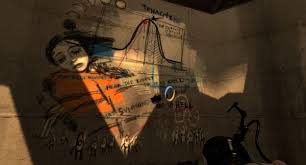
\includegraphics[width=0.6\textwidth]{chapters/15/images/Portal.png}
    \caption{Eine Grafik von dem beschrieben Portal Grafitti.}
    \label{UST-6}
\end{figure}

Im Gegensatz zu environmental Stortelling darf das indexcial Storytelling mit dem Spieler \hl{agieren | meinst du interagieren?}. Das bedeutet, dass das Spiel ihm helfen kann weiter zukommen \hl{|mach einen punkt und einen neuen satz aus "indem es den Spieler Tipps gibt." | so wie: Dies passiert über tipps} Die Steuerung kann auch durch ein Tutorial im Spiel erklärt werden. Aber auch durch Schilder oder Bücher die im Spiel verteilt sind können Storyinhalte besitzen. Ein gutes Beispiel wäre \verb+Super Mario 64+ \hl{mach die spiele immer als verb so wie ichs gemacht hab (falls du neue schreibst oder findest)} in dem der Spieler am Anfang ein Schild sieht, worin die Story als auch die Spielsteuerung erklärt wird. Wichtig bei der Methode ist, dass es nicht das Spielerlebnis durch zu viele Interaktionen mit dem Spieler verschlechtert. 

\subsection{Spannung einer Handlung}
Die Handlung eines Spiel sollte immer spannend gehalten werden. Aber der den Spieler nie überfordern. Wenn der Spieler überfordert ist, ist dieser genervt und kann nicht mehr das Spiel genießen. Aber die Story sollte auch nicht zu langweilig sein um das Spielerlebnis zu trüben. Zudem sollte die Handlung eines Spieles der eines Filmes gleichen. Damit ist gemeint, das es am Anfang einen Aufbau der Story gibt. Danach bleibt die Steigung anhaltend bis am Schluss wo jeder Plot aufgelöst wird. Dieses Verfahren wird in fast jedem literarischen Werk verwendet, ob Film, Buch oder sogar Theater Stück. Dieses Schema ist beliebt da es Spannung erzeugt und \hl{den Endverbraucher (Spieler, Leser, Zuschauer) and die Geschichte klammert| den endverbraucher klammert? klingt nicht gut}. 

\subsection{Spannung Gameplay}
Auch das \bettergls{gameplay}{1} muss eine gewisse Spannung haben. Wenn das Spiel zu leicht ist fühlt sich der Spieler unterfordert. Aber wenn das Spiel zu schwer ist er frustriert.\\\\
Wichtig ist das der \bettergls{flow}{2} optimal zum Spiel passt. \hl{Gehen davon} aus es ist ein Spiel für jüngere Verbraucher, dann darf das Spiel nicht zu schwer sein, \hl{da die Erfahrung mit Spielen einfach zu wenig vorhanden ist}. Aber wenn die Zielgruppe Personen sind, die sich mit Videospielen gut auskennen, dann sollten sie auch Herausgefordert werden. Damit sie nicht während des Spielens aufgrund des zu leichten Gameplay keine lust mehr bekommen das Spiel zu spielen. Wichtig ist aber, dass der Flow während des Spielverlaufs ändert. Am Anfang sollte das Spiel einfach gehalten sein. Damit der User einen leichten Start in das Spiel bekommt. Wenn sich der Spieler an die \bettergls{gamemechaniken}{3} gewöhnt hat, muss der Spieler mehr gefordert werden damit sein Interesse bleibt. \hl{Zudem fühlt sich das Spiel eintönig an, wenn immer die gleiche Herausforderung entgegen kommt. | komischer satz} In der folgenden Abbildung aus dem Buch \citetitle{GameDesign} kann man erkennen, dass der Flow sich während des Spiels verändern soll.

\todo{hast du das nicht schonmal geschrieben? bei spiel schwirigkeit?}

\begin{figure}[H]
    \centering
    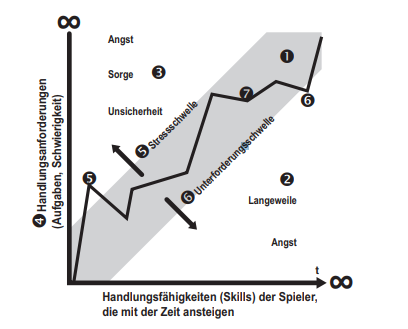
\includegraphics[width=0.8\textwidth]{chapters/15/images/GameFlow.png}
    \caption{Eine Grafik die den Flow verlauf des Spiels zeigt.}
    \label{UST-4}
\end{figure}


\subsection{Theme}
Das Theme ist dafür zuständig um die visuellen und audiodiven Reize des Spielers zu begeistern. Eine gute Story macht es nicht automatisch zu einem guten Spiel. Das Theme muss zur Story passen. In einem fröhlichen Spiel sind die Farben meist bunt und die Hintergrund-Musik sehr fröhlich und aufmunternd. Nicht wie bei einer düsteren beziehungsweise traurigen Story, da werden eher dunklere Farben und eine langsame umklammernde Musik verwendet. Das Theme muss den Spieler stimmig für die Story machen.

\todo{hast du das mit dem theme nicht auch schonmal geschrieben?}

\subsection{Spielidee für den Prototypen}
Für den Prototypen habe wir (Martin Usta und Lukas Schachinger) uns entschieden das wir einen \bettergls{platformer}{4} machen. \hl{Dieser Sollte beinhalten Sammelobjekte in Form von Münzen.} Aber auch schwierige Passagen in denen der Spieler sich gefordert fühlt. \hl{Der spielbare Charakter sollte auf jeden fall dynamische Animationen besitzen. | well...} Zudem sollten auch Gegner in diesem Spiel vorkommen, um den Spieler zu hindern das Ende zu erreichen. Die Inspiration für diese Art vom Spiel, war das damalige Kult Spiel \verb+Kao the Kangaro Round 2+ welches im November 2004 erschienen ist.\\\\

\subsection{Storyline für den Prototypen}
Unser Hautprotagonist \hl{ generischer Name } ist eingeschlafen und findet sich in eine Traumwelt als Eule wieder. Er muss alles versuchen um aus dieser Welt herauszukommen. Doch diese Aufgabe ist schwieriger als er es vermuten mag. Um dieses Ziel zu bewältigen muss der Spieler Fallen ausweichen, \hl{Rätsel lösen |wirklich?} und Gegener die ihm in den Weg stellen ausschalten. Dafür setzt er seine Eulenfähigkeiten ein. Ob ihm das gelingen wird ist nur eine Frage der Zeit. Aber er weiß, dass er muss so schnell wie möglich aufstehen um sein Kind vom Kindergarten abzuholen.

\begin{figure}[H]
    \centering
    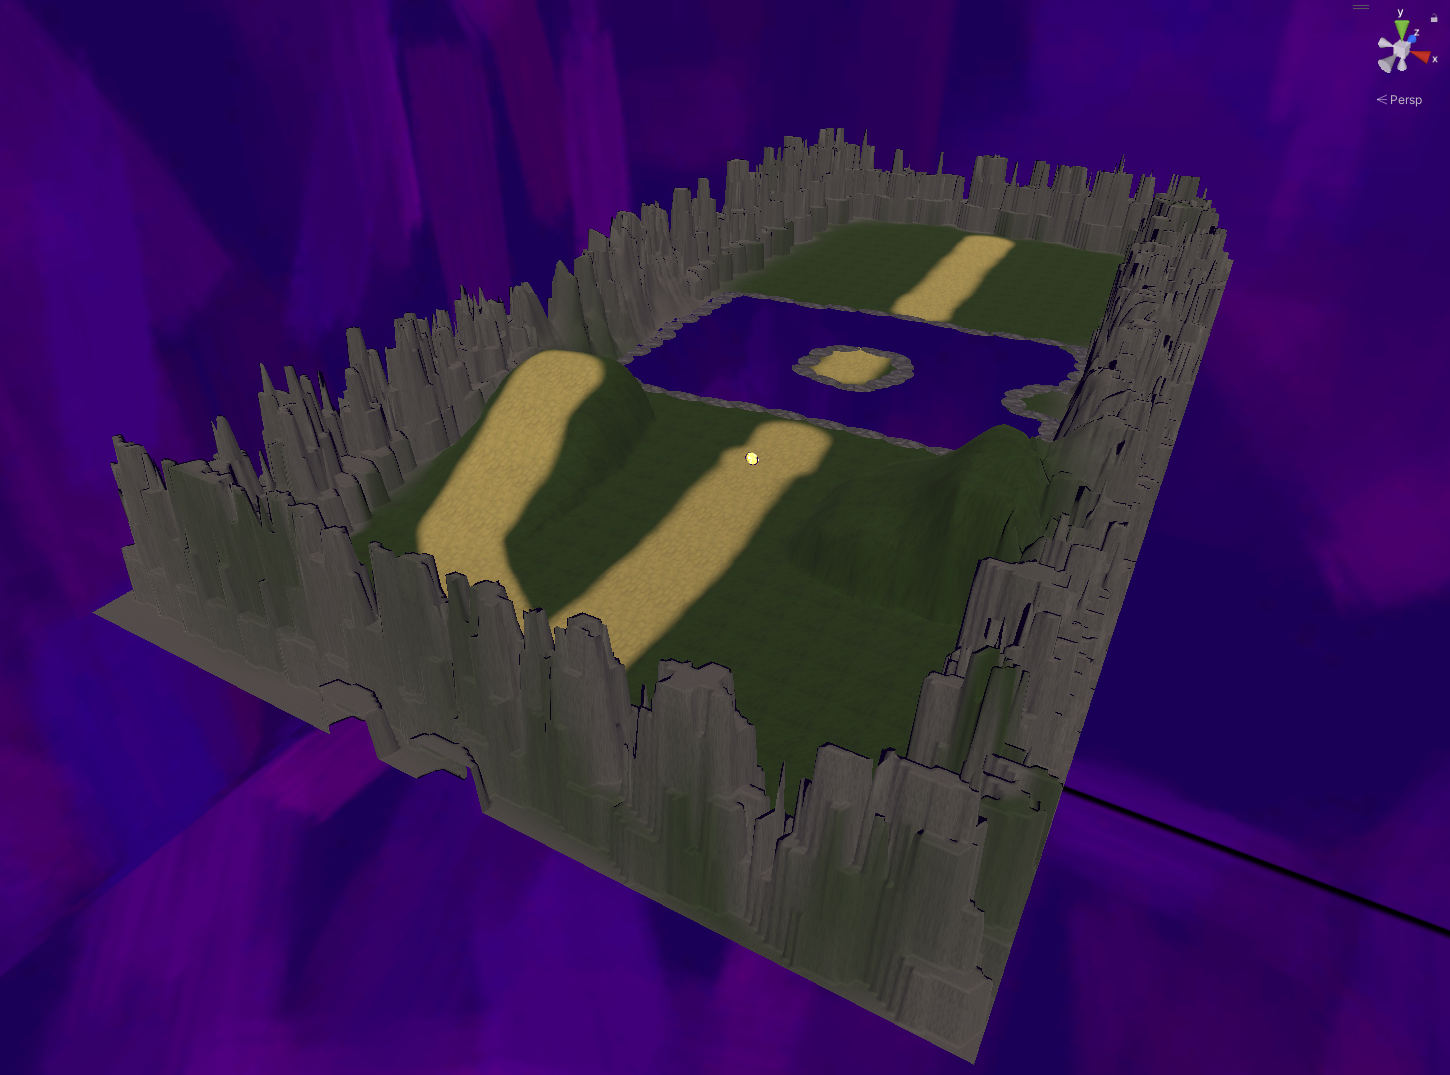
\includegraphics[width=0.8\textwidth]{chapters/15/images/Dreamworld.png}
    \caption{Eine Grafik des ersten Konzepts unsere Traumwelt.}
    \label{UST-7}
\end{figure}

